\section{Implementation}
\label{sec:impl}

\begin{figure}
  \centering
  \begin{tikzpicture}
    \tikzstyle{node} = [
      rectangle,rounded corners,minimum width=1.5cm,minimum height=1cm,text centered,
      draw=black,fill=red!80,align=center,anchor=west,font=\footnotesize
    ];
    \tikzstyle{input} = [trapezium, trapezium left angle=70, trapezium right angle=110, minimum width=1.5cm, minimum height=1cm, text centered, draw=black, fill=blue!30,align=center,anchor=west,font=\footnotesize];

    \node (loop) [input] at (0,0) {Input loop\\expression};
    \node (loopy) [node,at={(loop.east)},xshift=.7cm] {Generate\\loopy kernel};
    \node (c) [node,at={(loopy.east)},xshift=.7cm] {Generate\\C code};
    \node (exe) [node,at={(c.east)},xshift=.7cm] {Compile\\binary};
    \node (do) [node,at={(exe.east)},xshift=.7cm] {Execute};

    \draw [-{stealth}] (loop) -- (loopy);
    \draw [-{stealth}] (loopy) -- (c);
    \draw [-{stealth}] (c) -- (exe);
    \draw [-{stealth}] (exe) -- (do);
    \draw [-{stealth},densely dashed] (loop) to [bend left=35]
      node[midway,above,align=center,font=\footnotesize] {Pass in data from\\loop expression} (do);
  \end{tikzpicture}
  \caption{The code generation and execution pipeline for a \pyop3 loop expression.}
  \label{fig:codegenproc}
\end{figure}

\begin{listing}
  \begin{minted}{python}
do_loop(
  c := mesh.cells.index,
  kernel(dat0[closure(c)], dat1[closure(c)])
)
  \end{minted}
  \caption{\pyop3 code declaring and executing a loop expression for finite element-type computations (since \py{closure} is used).}
  \label{lst:pyop3_res_assembly}
\end{listing}

\begin{listing}
  \begin{minted}{c}
void do_loop(int ncells, double *dat0, double *dat1, int *map0) {
  double t0[CLOSURE_SIZE], t1[CLOSURE_SIZE];

  for (int c=0; c<ncells; ++c) {
    // Pack temporaries
    for (int p=0; p<CLOSURE_SIZE; ++p) {
      t0[p] = dat0[map0[c*CLOSURE_SIZE+p]];
      t1[p] = 0.0;
    }
    // Do the local computation
    kernel(t0, t1);
    // Now scatter the results
    for (int p=0; p<CLOSURE_SIZE; ++p) {
      dat1[map0[c*CLOSURE_SIZE+p]] += t1[p];
    }
  }
}
  \end{minted}
  \caption{
    Simplified version of code that would be generated by \pyop3 for the loop expression from Section~\ref{sec:impl_interface}.
    \clang{kernel} has access descriptors \py{READ} and \py{INC}, explaining the differing treatment for \clang{t0} and \clang{t1}.
    \clang{CLOSURE_SIZE} is an integer constant and would be known at compile-time.
  }
  \label{lst:basicloop}
\end{listing}

As discussed in Section~\ref{sec:stencillang}, existing stencil libraries may be classified according to whether or not they are aware of the mesh topology.
A library that is not `mesh-aware', for example \pyop2, can be more challenging to program in because responsibility for reasoning about the topology, including orientations, is passed to the user who has to construct the appropriate indirection maps to represent their mesh.
Composition of indirection maps is also difficult because of the loss of topological information.
Such difficulties can be avoided with a mesh-aware stencil library, but (usually) at the expense of relying upon a custom mesh abstraction implementation.
Writing mesh codes by hand is a non-trivial task requiring a significant amount of developer effort to maintain and introduce new features.
An in-house implementation will also never be able to compete with the feature set of a more general purpose mesh library (e.g. I/O, parallel decomposition, adaptive refinement) and will also suffer from poor interoperability with other packages.

In this work we attempt to bridge the gap between mesh-aware and mesh-oblivious stencil libraries by writing a new stencil library, \pyop3, that combines the advantages provided by mesh-aware frameworks with DMPlex, a mature, external mesh implementation (Section~\ref{sec:background_mesh_dmplex}).

\pyop3 is, somewhat obviously, heavily inspired by and based upon \pyop2, and hence much of its design represents either an incremental improvement on \pyop2, or is in fact directly lifted from it.
This report will make clear what parts of the design of \pyop3 are novel contributions and which are derived from \pyop2.

\subsection{Interface}
\label{sec:impl_interface}

\pyop3 is implemented as a \gls{dsl} embedded in Python.
As part of a larger script users create \textit{loop expressions}, prescribing the loops, local computations and stencil data access patterns in a manner resembling the algorithm's pseudocode.
These loop expressions are then parsed, compiled and executed by the \pyop3 backend.

To give an example, the syntax for a typical \gls{fem} residual assembly, where one loops over cells and computes using data in the cell's closure, would look something like the code shown in Listing~\ref{lst:pyop3_res_assembly}.
Here the function \py{do_loop} declares and then executes the loop expression.
All loop expressions consist of:
1) an iteration set, here \py{mesh.cells}, and
2) a sequence of instructions to execute, here simply the single local kernel \py{kernel}.
\py{kernel} has type \py{LocalKernel} and consists of a \textit{loopy kernel} (Section~\ref{sec:impl_interface_codegen}) augmented with \textit{access descriptors} for each of its arguments.
Possible access descriptors are \py{READ}, \py{WRITE}, \py{RW}, \py{INC}, \py{MIN} and \py{MAX} and they are required to ensure that \pyop3 generates the right packing/unpacking code.
An example for a kernel with access descriptors \py{READ} and \py{INC} is shown in Listing~\ref{lst:basicloop}.
Lastly, the \py{dat{0,1}[closure(c)]} instructions indicate that \py{kernel} should be passed two contiguous arrays, each containing the \glspl{dof} associated with the closure of the current cell.
This last part is where the difference between the mesh-oblivious \pyop2 and the mesh-aware \pyop3 is stark.
In \pyop2 these closure maps would need to be computed in advance and passed in to the loop expression whereas \pyop3, being mesh-aware, is capable of reasoning about the mesh and automatically computing the right indirection maps.

Note that in this example, by using \py{do_loop}, we declare the loop expression and then \textit{immediately execute it}.
This is not always desired behaviour as, if the same loop expression is executed multiple times, one may want to have a \textit{persistent} loop expression to avoid some overhead.
Such expressions can easily be created by calling \py{expr = loop(...)}, and then executed with Python call syntax: \py{expr(*args, **kwargs)}.
This is discussed in more detail in Section~\ref{sec:impl_overhead}.

\subsubsection{Code generation}
\label{sec:impl_interface_codegen}

Having declared a loop expression, \pyop3 executes it by first lowering the expression through a sequence of intermediate representations, compiling to a binary, then running the code.

The target intermediate representation of \pyop3 is loopy~\cite{klocknerLooPyTransformationbased2014}, a polyhedral model inspired Python code generation library capable of generating code for multiple backends including CPUs and GPUs.
With loopy, the main entry point is, not dissimilarly to \pyop3, the declaration of a \py{LoopKernel} via the command \py{loopy.make_kernel}.
Once a \py{LoopKernel} has been created, loopy also provides a wealth of different code transformations such as loop tiling, vectorisation and loop-invariant code motion.

To construct such a kernel, the user needs to specify \textit{domains}, effectively loop extents, \textit{instructions} (e.g. \clang{x[i] += y[i]}) and \textit{arguments} representing kernel inputs.
For example, a simple loopy kernel could be created as follows:

\vspace{1em}
\begin{minipage}{\textwidth}
\begin{minted}[xleftmargin=2em]{python}
knl = loopy.make_kernel(
  "{ [i]: 0 <= i < n }",  # domains
  "y[i] = 2*x[i]",        # instructions
  [                       # arguments
    loopy.GlobalArg("x"),
    loopy.GlobalArg("y"),
    loopy.ValueArg("n"),
  ],
)
\end{minted}
\end{minipage}
\vspace{1em}

The role of \pyop3 in lowering to such a representation is therefore to determine the correct number and size of the iteration domains, and resolving the complex data access patterns required for multi-dimensional mesh data in order to emit the correct instructions.

Once \pyop3 has generated an appropriate loopy kernel, loopy is called upon to generate code in a low-level device-specific language (e.g. C for CPUs).
This code is then compiled by \pyop3 and executed.
A high-level overview of the code generation pathway is shown in Figure~\ref{fig:codegenproc} and an example of the sort of C code that would be emitted is shown in Listing~\ref{lst:basicloop}.

\subsubsection{Data types}

Just like \pyop2, \pyop3 has three main data types:
\py{Globals}, values shared across all processors;
\py{Dats}, vectors storing data associated with mesh points;
and \py{Mats}, matrices (usually sparse) representing interactions between mesh points.

The distribution of these parallel objects is discussed in Section~\ref{sec:impl_parallel}.

\subsection{A new abstraction for mesh data layouts}
\label{sec:impl_datalayout}

\begin{figure}
  \centering
  \begin{subfigure}[t]{0.48\textwidth}
    \centering
    \begin{tikzpicture}[y=-1cm,scale=.75]
      \begin{scope}[yshift=0cm]
        \fill[lightgray] (0,0) rectangle(6,1);
        \filldraw[draw=black, fill=white] (0.5,0) rectangle ++ (1,1);
        \filldraw[draw=black, fill=white] (1.5,0) rectangle ++ (1,1);
        \filldraw[draw=black, fill=white] (2.5,0) rectangle ++ (1,1);
        \filldraw[draw=black, fill=white] (3.5,0) rectangle ++ (1,1);
        \filldraw[draw=black, fill=white] (4.5,0) rectangle ++ (1,1);
        \node[at={(1,.5)}, ptlabel] {$i_0$};
        \node[at={(2,.5)}, ptlabel] {$i_1$};
        \node[at={(3,.5)}, ptlabel] {$i_4$};
        \node[at={(4,.5)}, ptlabel] {$i_5$};
        \node[at={(5,.5)}, ptlabel] {$i_9$};
        \draw (0,0) -- (6,0);
        \draw (0,1) -- (6,1);
      \end{scope}

      \begin{scope}[xshift=1.5cm,yshift=-2cm]
        \filldraw[draw=black, fill=white] (0,0) rectangle ++ (1,1);
        \filldraw[draw=black, fill=white] (1,0) rectangle ++ (1,1);
        \filldraw[draw=black, fill=white] (2,0) rectangle ++ (1,1);
        \node[at={(0.5,.5)}, ptlabel] {$d_0$};
        \node[at={(1.5,.5)}, ptlabel] {$d_1$};
        \node[at={(2.5,.5)}, ptlabel] {$d_2$};

        \draw (1,-1) -- (0,0);
        \draw (2,-1) -- (3,0);
      \end{scope}

      \node (nodeslabel) [ptlabel] at (7,.5) {Nodes};
      \node (dofslabel) [ptlabel] at (7,2.5) {\glspl{dof}};
    \end{tikzpicture}
    \caption{
      A typical \pyop2 \py{Dat} data layout for a \py{DataSet} with \py{dim} \py{(3,)}.
      Note that the nodes are unordered, since we are on an unstructured mesh, but that the \glspl{dof} are ordered.
    }
    \label{fig:vdat_pyop2}
  \end{subfigure}
  \hfill
  \begin{subfigure}[t]{0.48\textwidth}
    \centering
    \begin{tikzpicture}[y=-1cm,scale=.75]
      \begin{scope}[yshift=0cm]
        \fill[lightgray] (0,0) rectangle(6,1);
        \filldraw[draw=black, fill=white] (0.5,0) rectangle ++ (1,1);
        \filldraw[draw=black, fill=white] (1.5,0) rectangle ++ (1,1);
        \filldraw[draw=black, fill=white] (2.5,0) rectangle ++ (1,1);
        \filldraw[draw=black, fill=white] (3.5,0) rectangle ++ (1,1);
        \filldraw[draw=black, fill=white] (4.5,0) rectangle ++ (1,1);
        \node[at={(1,.5)}, ptlabel] {$c_5$};
        \node[at={(2,.5)}, ptlabel] {$v_1$};
        \node[at={(3,.5)}, ptlabel] {$e_4$};
        \node[at={(4,.5)}, ptlabel] {$e_5$};
        \node[at={(5,.5)}, ptlabel] {$c_9$};
        \draw (0,0) -- (6,0);
        \draw (0,1) -- (6,1);
      \end{scope}

      \begin{scope}[xshift=2cm,yshift=-2cm]
        \filldraw[draw=black, fill=white] (0,0) rectangle ++ (1,1);
        \filldraw[draw=black, fill=white] (1,0) rectangle ++ (1,1);
        \node[at={(0.5,.5)}, ptlabel] {$i_0$};
        \node[at={(1.5,.5)}, ptlabel] {$i_1$};

        \draw (.5,-1) -- (0,0);
        \draw (1.5,-1) -- (2,0);
      \end{scope}

      \begin{scope}[xshift=1cm,yshift=-4cm]
        \filldraw[draw=black, fill=white] (0,0) rectangle ++ (1,1);
        \filldraw[draw=black, fill=white] (1,0) rectangle ++ (1,1);
        \filldraw[draw=black, fill=white] (2,0) rectangle ++ (1,1);
        \node[at={(0.5,.5)}, ptlabel] {$d_0$};
        \node[at={(1.5,.5)}, ptlabel] {$d_1$};
        \node[at={(2.5,.5)}, ptlabel] {$d_2$};

        \draw (1,-1) -- (0,0);
        \draw (2,-1) -- (3,0);
      \end{scope}

      \node (pointslabel) [ptlabel] at (7,.5) {Points};
      \node (nodeslabel) [ptlabel] at (7,2.5) {Nodes};
      \node (dofslabel) [ptlabel] at (7,4.5) {\glspl{dof}};
    \end{tikzpicture}
    \caption{
      The equivalent \pyop3 data layout that is aware of the topology of the mesh.
      Note that the number of nodes per entity is not constant - here we indicate that there are 2 nodes per edge but this may differ for cells and vertices.
    }
    \label{fig:vdat_pyop3}
  \end{subfigure}
  \caption{Comparing the \gls{dof} layouts for a vector-valued \py{Dat} between \pyop2 (left) and \pyop3 (right).}
  \label{fig:vdat_comparison}
\end{figure}

\begin{figure}
  \centering
  \begin{subfigure}{.9\textwidth}
    \centering
    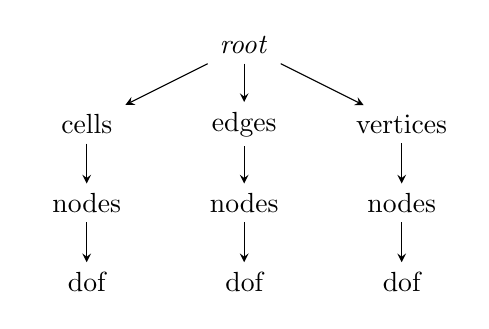
\begin{tikzpicture}
      \tikzstyle{node} = [minimum width=1.5cm,text centered,align=center];

      \node [node] (root) at (0,0) {\textit{root}};
      \node [node] (cells) at (-2,-1) {cells};
      \node [node] (edges) at (0,-1) {edges};
      \node [node] (verts) at (2,-1) {vertices};
      \node [node] (cnodes) at (-2,-2) {nodes};
      \node [node] (enodes) at (0,-2) {nodes};
      \node [node] (vnodes) at (2,-2) {nodes};
      \node [node] (cdofs) at (-2,-3) {\glspl{dof}};
      \node [node] (edofs) at (0,-3) {\glspl{dof}};
      \node [node] (vdofs) at (2,-3) {\glspl{dof}};

      \draw [-{stealth}] (root) -- (cells);
      \draw [-{stealth}] (root) -- (edges);
      \draw [-{stealth}] (root) -- (verts);
      \draw [-{stealth}] (cells) -- (cnodes);
      \draw [-{stealth}] (edges) -- (enodes);
      \draw [-{stealth}] (verts) -- (vnodes);
      \draw [-{stealth}] (cnodes) -- (cdofs);
      \draw [-{stealth}] (enodes) -- (edofs);
      \draw [-{stealth}] (vnodes) -- (vdofs);
    \end{tikzpicture}
    \caption{
      An example data layout tree.
      Each node in the tree, excluding \textit{root}, corresponds to a \pyop3 \py{AxisPart}.
    }
    \label{fig:vdat_tree}
  \end{subfigure}
  
  \vspace{1em}

  \begin{subfigure}{.9\textwidth}
    \begin{minted}[xleftmargin=4em,fontsize=\footnotesize]{python}
root = (
  MultiAxis()
  .add_part(AxisPart(ncells, id="cells"))
  .add_part(AxisPart(nedges, id="edges"))
  .add_part(AxisPart(nverts, id="verts"))
  .add_subaxis("cells", AxisPart(ncnodes, id="cnodes"))
  .add_subaxis("edges", AxisPart(nenodes, id="enodes"))
  .add_subaxis("verts", AxisPart(nvnodes, id="vnodes"))
  .add_subaxis("cnodes", AxisPart(ncdofs))
  .add_subaxis("enodes", AxisPart(nedofs))
  .add_subaxis("vnodes", AxisPart(nvdofs))
)
    \end{minted}
    \caption{
      \pyop3 code for constructing the tree structure shown above.
      \py{ncells}, \py{ncnodes} etc are integers and correspond to the number of entries for a given \py{AxisPart}.
    }
    \label{lis:demotreecode}
  \end{subfigure}
  \caption{Example hierarchical data layout for a \py{Dat} in \pyop3.}
  \label{fig:demotree}
\end{figure}

The additional flexibility \pyop3 has over \pyop2 is thanks to its novel abstraction for describing data layouts.

In \pyop2, data layouts are prescribed by associating data (i.e. \glspl{dof}) with \textit{sets}.
More precisely, they are described using a \py{DataSet}, which is formed by associating a \py{Set} with some \textit{local shape} (a tuple), termed its \py{dim}.
An example of this is shown in Figure~\ref{fig:vdat_pyop2}.
The \py{Set} here consists of the nodes in the mesh and the \py{dim} is \py{(3,)}, thus every node in the mesh stores 3 entries.

The fundamental idea behind \pyop3 is the observation that such a two-layered data layout is insufficient for fully describing the complexities of data living on an unstructured mesh; in particular, \textit{topological information is lost}.
Typical \py{Dats} in \pyop2 use the \textit{nodes} of the mesh to form the underlying \py{Set}.
Recalling from Section~\ref{sec:background_mesh} that the nodes of a mesh are associated with a particular topological entity (i.e. cells, edges, etc), using nodes as a basis for describing a data layout means that information about the topological entities these nodes come from is lost.
We claim that this `premature flattening' of the data layout is disadvantageous, and so \pyop3 aims for a more complete description of it.

In order to do so, \pyop3 replaces the two-layered \py{DataSet} abstraction with a hierarchical, tree-based data layout.
Each layer of the hierarchy (e.g. topological entities or nodes) is represented by a \py{MultiAxis} object, and to each \py{MultiAxis} is associated one or more \py{AxisParts}.
\py{AxisParts} correspond to a particular `class' of entity stored in the \py{MultiAxis} and, for instance, allow \pyop3 to differentiate between the cells, edges and vertices of the mesh.
An example of such a data layout is shown in Figure~\ref{fig:vdat_pyop3}.
Compared with the equivalent \pyop2 data layout in Figure~\ref{fig:vdat_pyop2}, one can immediately see how topological information is preserved via the addition of an extra ``Points" \py{MultiAxis}.
Since the mesh will have been renumbered to improve data locality (Section~\ref{sec:background_opt_locality}), entries from different \py{AxisParts} (cells, edges and vertices) need to be interleaved.

To construct the hierarchy, it is permitted to attach a new \py{MultiAxis} to each \py{AxisPart}.
The interface for this, and the resulting tree structure, is shown in Figure~\ref{fig:demotree}.

The hierarchical data layout system described here is similar to that used in Taichi~\cite{huTaichiLanguageHighperformance2019}, though Taichi does not support interleaving components of an axis as we do here.
It also has no support for distributed memory parallelism (see Section~\ref{sec:impl_parallel}).

\subsubsection{Addressing the inhomogeneous}

One major challenge presented by this new abstraction is that axes are no longer homogeneous.
Previously, in \pyop2, one could stride over a \py{Dat} with steps matching the size of its \py{dim}.
This is no longer possible since the strides for, say, the ``Points" \py{MultiAxis} in Figure~\ref{fig:vdat_pyop3} are not constant because the number of nodes stored can differ between topological entities.
Addressing individual topological entities therefore requires careful thought and in \pyop3 is separated into two phases:
1) entries in the data layout are addressed with \textit{typed multi-indices}, and
2) these multi-indices are composed with \textit{layout functions} to determine the correct offset into the data.

To start with the former, a typed multi-index is an object of the form $(t^0_{i_0}, t^1_{i_2}, \dots, t^n_{i_n})$ with $t^x$ indicating the `type' of index $i_y$.
The type is required to select the correct \py{AxisPart} from a particular \py{MultiAxis}, and the index indicates which entry of that type is to be selected.
To give an example, in order to correctly address the $d_0$ entry from Figure~\ref{fig:vdat_pyop3}, the multi-index $(e_4, i_0, d_0)$.
Similarly, for the code shown in Listing~\ref{lst:pyop3_res_assembly}, \py{mesh.cells.index} is a multi-index selecting all cells in the mesh.
\py{closure(c)} is in fact a \textit{map} and represents a collection of multi-indices.

Provided with a multi-index, we can now use the appropriate layout functions to determine the right memory address (offset) for the data.
In \pyop3, layout functions are simply functions that take one or more indices and return an offset value. 
For example, in the case of axes with constant strides, a layout function would be some affine function of the form \clang{offset = i*stride + step} (with \clang{i} the input index).
If the axis has non-constant strides then the layout function instead needs to be some sort of lookup table (i.e. \clang{offset = offsets[i]}).

Layout functions are associated with individual \py{AxisParts} and so the process of determining the correct offset for a given multi-index is as follows:

\begin{enumerate}
  \item
    Each `type' in the multi-index is used to select a particular \py{AxisPart} in the hierarchy.

  \item
    The index part of the multi-index entry is then passed to the layout function of the selected \py{AxisPart} to compute an offset value.

  \item
    The offsets for each level of the hierarchy are added together, yielding the final memory address.
\end{enumerate}

\subsubsection{Maps}
\label{sec:impl_datalayout_maps}

\begin{listing}
  \begin{minted}{python}
do_loop(
  f := mesh.interior_facets.index,
  kernel(
    dat0[closure(support(f))],
    dat1[closure(support(f))]
  )
)
  \end{minted}
  \caption{Example \pyop3 code for computations over the cells incident on an interior facet.}
  \label{lst:pyop3_intfacet}
\end{listing}

As previously mentioned, \py{closure(c)} from Listing~\ref{lst:pyop3_res_assembly} is an example of a \textit{map}, a function from one multi-index to many multi-indices.
With a mesh of triangles, \py{closure(c)} would correspond to a function like:

\begin{equation*}
  (c_i,)
  \to \big[
  (c_i,)
  ,\ (e_{j_0},) ,\ (e_{j_1},) ,\ (e_{j_2},)
  ,\ (v_{j_3},) ,\ (v_{j_4},) ,\ (v_{j_5},) \big] .
\end{equation*}

In other words, \py{closure(c)} yields, for every cell, 7 multi-indices pointing to the cell and the 6 incident edges and vertices.

In an identical way to layout functions, maps can be implemented either using affine functions (i.e. \clang{e_0 = c_0*step + start}), or lookup tables (i.e. \clang{e0 = map[c0]}) depending on whether or not there is structure to exploit in the data layout.
This enables, for example, the use of structured meshes without needing to incur the data volume/memory bandwidth cost of tabulating a lookup table.

The approach just described enables arbitrary map composition because maps now relate mesh points to mesh points, rather than mesh points to nodes as is done in \pyop2.
\todo{Could include a commutativity diagram to make this clearer.}
This is also the approach done by DMPlex.

An example of this map composition is shown in Listing~\ref{lst:pyop3_intfacet}.
\pyop3 makes it easy to describe more complex stencils such as for interior facet-type computations where the stencil consists of the closure of the cells incident on a facet, or, in DMPlex terminology, $\closure(\support(p))$.

Note that thus far we have only discussed maps in the context of mapping between multi-indices containing just a single typed index.
It is entirely possible to map between multi-indices with two or more entries, but we require that any `parent' indices of the map outputs are the same as those for the map input.
This is sufficient for unstructured meshes but not for partially-structured meshes (see Section~\ref{sec:future_partialstructure_maps}).
We similarly require that maps only relate multi-indices of the same size.
\todo{These could be demonstrated with an example.}

\subsubsection{Raggedness}
\label{sec:impl_datalayout_ragged}

There are occasions where one needs a data structure where the extent of an inner dimension depends on an outer one.
This occurs for example in variable layer extruded meshes (Section~\ref{sec:future_partialstructure}) - the extent of the inner dimension (the columns) is dependent upon the mesh point in the base mesh.
To get this to work, \pyop3 needs to generate code that resembles:

\begin{minted}[xleftmargin=4em]{c}
for (int i=0; i<N; ++i)
  for (int j=0; j<nlayers[i]; ++j)
    ...
\end{minted}

Note how the inner loop extent is dependent upon the outer one via the \clang{nlayers} array.

In \pyop3, such a `ragged' data structure can be initialised in the following way:

\vspace{1em}
\begin{minipage}{\textwidth}
\begin{minted}[xleftmargin=4em]{python}
# store nlayers as an integer Dat
nlayers = Dat(MultiAxis(AxisPart(N)), dtype=int)
# nlayers is used as the extent of the 'inner' axis
root = (
  MultiAxis()
  .add_part(AxisPart(N, id="outer"))
  .add_subaxis("outer", AxisPart(nlayers))
)
\end{minted}
\end{minipage}
\vspace{1em}

Instead of using a constant integer value to prescribe the extent of the inner \py{AxisPart}, a \py{Dat}, \py{nlayers}, is used instead.

We can also use the same technique to generate code for maps with \textit{variable arity}.
An example of this would be for $\plexstar(v)$ with $v$ a vertex since the number of incident edges on a vertex can vary.
\todo{Should provide more demo code}
This is useful for patch-based computations (see Section~\ref{sec:future_patch}).

\subsubsection{Sparsity}
\label{sec:impl_datalayout_sparsity}

Although not yet implemented, it should be entirely possible to implement sparse data structures by making small extensions to the existing abstraction.
If we consider a sparse matrix compressed with compressed-sparse-row (CSR) format, the data layout is described using two arrays: the row and column indices.
This is very similar to our existing solution for ragged arrays above except that we assume that the internal dimension is logically dense, and hence do not need to specify column indices.
\todo{Would be served well by an example}

\subsubsection{Orienting degrees-of-freedom}
\label{sec:impl_orientation}

% an advantage we have over Basix is we differentiate between nodes and dofs so can transform them
% separately. transformation matrices are very very small.

Having a hierarchical, `mesh-aware' data layout makes it straightforward to correctly handle orientations when packing stencils.
In \pyop3 we can augment maps to return orientation information along with each multi-index.
Using the triangles from Figure~\ref{fig:orient} as an example, the edges of the `canonical' triangles would have orientations $(0,0,0)$, whilst the edges of the triangles with one flipped edge would have orientations $(0,0,-1)$.

To handle the \gls{dof} transformations required for correctly orienting things, \pyop3 can apply a different transformation on each \py{AxisPart}.
For instance if the nodes are out of order then \pyop3 can apply a permutation to the entries of the \py{AxisPart} (though in practice this would likely be done when preparing the maps), and if the \glspl{dof} require a transformation then this can be applied to the corresponding \py{AxisPart}.
\todo{A demo would help}

\subsubsection{Data layout transformations}
\label{sec:impl_datalayoutopt}

\begin{figure}
  % macros
  \newcommand{\mixedstylesetup}{%
    \tikzstyle{v0} = [fill=blue!50];
    \tikzstyle{v1} = [fill=red!65];
  }

  \centering
  \begin{subfigure}{.65\textwidth}
    \centering
    \begin{tikzpicture}[y=-1cm,scale=.75]
      \mixedstylesetup
      \begin{scope}[xshift=3.25cm, yshift=0cm]
        \filldraw[v0,draw=black] (0,0) rectangle (1,1);
        \filldraw[v1,draw=black] (1,0) rectangle (2,1);
        \node[at={(.5,.5)}, ptlabel] {$V_0$};
        \node[at={(1.5,.5)}, ptlabel] {$V_1$};
      \end{scope}

      \begin{scope}[yshift=-2cm]
        \begin{scope}[xshift=0cm]
          \fill[lightgray] (0,0) rectangle (4,1);
          \filldraw[draw=black, fill=white] (0.5,0) rectangle (1.5,1);
          \filldraw[draw=black, fill=white] (1.5,0) rectangle (2.5,1);
          \filldraw[draw=black, fill=white] (2.5,0) rectangle (3.5,1);
          \node[at={(1,.5)}, ptlabel] {$c_0$};
          \node[at={(2,.5)}, ptlabel] {$v_1$};
          \node[at={(3,.5)}, ptlabel] {$c_4$};
          \draw (0,0) -- (4,0);
          \draw (0,1) -- (4,1);
        \end{scope}

        \begin{scope}[xshift=4.5cm]
          \fill[lightgray] (0,0) rectangle (4,1);
          \filldraw[draw=black, fill=white] (0.5,0) rectangle (1.5,1);
          \filldraw[draw=black, fill=white] (1.5,0) rectangle (2.5,1);
          \filldraw[draw=black, fill=white] (2.5,0) rectangle (3.5,1);
          \node[at={(1,.5)}, ptlabel] {$c_0$};
          \node[at={(2,.5)}, ptlabel] {$v_1$};
          \node[at={(3,.5)}, ptlabel] {$c_4$};
          \draw (0,0) -- (4,0);
          \draw (0,1) -- (4,1);
        \end{scope}
      \end{scope}

      \draw [densely dashed] (3.25,1) -- (0,2);
      \draw [densely dashed] (4.25,1) -- (4,2);
      \draw [densely dashed] (4.25,1) -- ({0+4.5},2);
      \draw [densely dashed] (5.25,1) -- ({4+4.5},2);

      \node [at={(9.5,.5)},anchor=center] {Spaces};
      \node [at={(9.5,2.5)},anchor=center] {Points};
    \end{tikzpicture}
    \caption{
      A typical data layout for a `mixed' system with the spaces $V_0$ and $V_1$ forming the `outer' axis.
    }
    \label{fig:mixedreorder_outer}
  \end{subfigure}
  \hfill
  \begin{subfigure}{.3\textwidth}
    \centering
    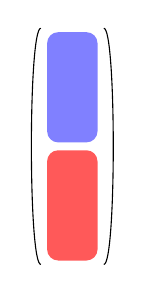
\begin{tikzpicture}[x=.8cm,y=-1cm]
      \mixedstylesetup
      \draw (0,0) .. controls (-.2,0) and (-.2,3) .. (0,3);
      \draw (1,0) .. controls (1.2,0) and (1.2,3) .. (1,3);
      \filldraw [v0,rounded corners,draw=none]
        (.1,.05) -- (.9,.05) -- (.9,1.45) -- (.1,1.45) -- cycle;
      \filldraw [v1,rounded corners,draw=none]
        (.1,1.55) -- (.9,1.55) -- (.9,2.95) -- (.1,2.95) -- cycle;
    \end{tikzpicture}
    \caption{The resulting block-structured vector.}
    \label{fig:mixedreorder_outer_vec}
  \end{subfigure}

  \vspace{1em}
 
  \begin{subfigure}{.65\textwidth}
    \centering
    \begin{tikzpicture}[y=-1cm,scale=.75]
      \mixedstylesetup
      \begin{scope}[xshift=0cm,yshift=0cm]
        \fill[lightgray] (0,0) rectangle (4,1);
        \filldraw[draw=black, fill=white] (0.5,0) rectangle (1.5,1);
        \filldraw[draw=black, fill=white] (1.5,0) rectangle (2.5,1);
        \filldraw[draw=black, fill=white] (2.5,0) rectangle (3.5,1);
        \node[at={(1,.5)}, ptlabel] {$c_0$};
        \node[at={(2,.5)}, ptlabel] {$v_1$};
        \node[at={(3,.5)}, ptlabel] {$c_4$};
        \draw (0,0) -- (4,0);
        \draw (0,1) -- (4,1);
      \end{scope}

      \begin{scope}[xshift=1cm, yshift=-2cm]
        \filldraw[v0,draw=black] (0,0) rectangle (1,1);
        \filldraw[v1,draw=black] (1,0) rectangle (2,1);
        \node[at={(.5,.5)}, ptlabel] {$V_0$};
        \node[at={(1.5,.5)}, ptlabel] {$V_1$};
      \end{scope}

      \draw (1.5,1) -- (1,2);
      \draw (2.5,1) -- (3,2);

      \node [at={(5,.5)},anchor=center] {Points};
      \node [at={(5,2.5)},anchor=center] {Spaces};
    \end{tikzpicture}
    \caption{A transformed data layout where the ``Spaces" and ``Points" axes have been swapped.}
    \label{fig:mixedreorder_inner}
  \end{subfigure}
  \hfill
  \begin{subfigure}{.3\textwidth}
    \centering
    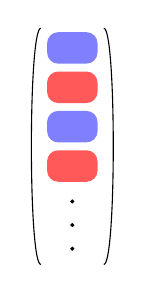
\begin{tikzpicture}[x=.8cm,y=-1cm]
      \mixedstylesetup
      \tikzstyle{entry} = [rounded corners,draw=none];
      \tikzstyle{blue} = [v0,entry];
      \tikzstyle{red} = [v1,entry];
      \draw (0,0) .. controls (-.2,0) and (-.2,3) .. (0,3);
      \draw (1,0) .. controls (1.2,0) and (1.2,3) .. (1,3);
      \filldraw [blue] (.1,.05) -- (.9,.05) -- (.9,.45) -- (.1,.45) -- cycle;
      \filldraw [red] (.1,.55) -- (.9,.55) -- (.9,.95) -- (.1,.95) -- cycle;
      \filldraw [blue] (.1,1.05) -- (.9,1.05) -- (.9,1.45) -- (.1,1.45) -- cycle;
      \filldraw [red] (.1,1.55) -- (.9,1.55) -- (.9,1.95) -- (.1,1.95) -- cycle;
      % \filldraw [blue] (.1,2.05) -- (.9,2.05) -- (.9,2.45) -- (.1,2.45) -- cycle;
      % \filldraw [red] (.1,2.55) -- (.9,2.55) -- (.9,2.95) -- (.1,2.95) -- cycle;
      % ellipsis
      \filldraw [fill=black] (.5,2.2) circle (.5pt);
      \filldraw [fill=black] (.5,2.5) circle (.5pt);
      \filldraw [fill=black] (.5,2.8) circle (.5pt);
    \end{tikzpicture}
    \caption{The resulting interleaved vector.}
    \label{fig:mixedreorder_inner_vec}
  \end{subfigure}
  \caption{
    A possible data layout transformation for a `mixed' system permitted by \pyop3.
    The entries $V_0$ and $V_1$ represent the spaces of the mixed system and the ``Points" axis is representative of the mesh.
    Note that additional subaxes for, for example, nodes and \glspl{dof} would be permitted.
  }
  \label{fig:mixedreorder}
\end{figure}

With this decomposition of data layouts in a flexible, declarative hierarchy, it is now relatively easy to make \textit{data layout transformations} to improve data locality (Section~\ref{sec:background_opt_locality}).
Some of the possible optimisations include:

\begin{paragraph}{Swapping axes}
\pyop3 allows the user to swap a pair of \py{MultiAxes} such that the `inner' axis becomes the `outer' and vice versa.
This can improve data locality if different entries from the outer axis are accessed in the same iteration.

An example of this is shown in Figure~\ref{fig:mixedreorder}.
Typically a `mixed' system like this - here formed of $V_0$ and $V_1$ - stores data in a blocked format (Figures~\ref{fig:mixedreorder_outer} and~\ref{fig:mixedreorder_outer_vec}).
This means that the \glspl{dof} corresponding to the same mesh point for $V_0$ and $V_1$ are very far apart in memory.
If they are both used in the local computation then this constitutes poor data locality.

To rectify the situation, we can swap the axes such that the mixed components are stored per mesh point, adjacent in memory.
This is shown in Figures~\ref{fig:mixedreorder_inner} and~\ref{fig:mixedreorder_inner_vec}.
\end{paragraph}

\begin{paragraph}{Reordering data within axes}
Once the axes have been ordered in the most advantageous way, we can now begin to rearrange the entries in a \py{MultiAxis} to maximise locality.
In the context of meshes, these reorderings could correspond to, for example, an \gls{rcm} renumbering of the mesh entities or a different ordering of the elements up the columns of an extruded mesh.
As well as to improve data locality, there are circumstances where the user may wish to prescribe a custom data layout specific to their problem.
For example, certain fieldsplit preconditioners may require a subset of \glspl{dof} to work, and performance could be improved by storing this subset as a contiguous block of memory.

To implement this reordering, \pyop3 simply requires that a different layout function be associated with the respective \py{AxisParts}.
Layout functions map entities in an axis to their offsets in memory and so using a different one gives the user total freedom over where data is stored.
This approach is roughly equivalent to permuting a \clang{PetscSection} in PETSc, though in our case we permit layout functions to be affine functions as well as tabulations.
\end{paragraph}

\subsubsection{Other locality optimisations}

\pyop3's abstraction also enables code transformations such as vectorisation and time-tiling (Section~\ref{sec:background_opt_locality}).
Such optimisations are not data layout transformations, but transformations of the \textit{iteration set}.
To enact such transformations, the iteration over the set needs to be broken into a nest of loops.
This would look something like:

\begin{minipage}{\textwidth}
\begin{minted}[xleftmargin=4em]{c}
for (int i=0; i<NOUTER; ++i) {
  for (int j=0; j<NINNER; ++j) {
    int k = i*NINNER + j;
    ...
  }
}
\end{minted}
\end{minipage}

In the case of vectorisation, \clang{NINNER} would correspond to the length of the vector lanes of the CPU.
If time-tiling, the size of tiles should be chosen such that data required for the fused kernels remain in cache between their invocations.

\subsubsection{Enabling new research}

In addition to the benefits espoused above, \pyop3's data layout abstraction should enable a number of new mathematical methods that would be very hard to impossible to implement in \pyop2.
These include:

\begin{itemize}
  \item
    \textbf{p-adaptivity}
    In order to reduce the errors in a simulation, one may vary the polynomial degree of particular cells in a process known as p-adaptivity.
    This introduces difficulties for stencil codes because:
    a) multiple local kernels are needed, one for each polynomial degree; and
    b) there are `hanging' nodes at the boundaries between cells of differing degrees.
    \todo{Provide example}

    Problem (a) is trivial to resolve in \pyop3.
    Rather than having a \py{MultiAxis} that is composed only of cells, edges and vertices (each a distinct \py{AxisPart}), additional \py{AxisParts} can be added such that mesh points of different degree are associated with a unique \py{AxisPart}.
    This would mean that points would no longer be addressed with multi-indices containing typed indices of the form $c_i$, $e_i$ and $v_i$, but instead be addressed with $c^d_i$, $e^d_i$ and $v^d_i$, where $d$ corresponds to the polynomial degree of the entity.

    Problem (b) is more challenging to solve and requires the addition of \textit{constraints} to the abstraction\footnote{This is the approach used by libCEED: \url{https://libceed.org/en/latest/libCEEDapi/\#finite-element-operator-decomposition}.}.
    Adding constraints would also enable \textit{adaptive mesh refinement}.
    Support for constraints has already been implemented for DMPlex~\cite{isaacSupportNonconformalMeshes2015}.

  \item
    \textbf{Mixed meshes}
    A mixed mesh is a mesh containing multiple different types of cell (e.g. triangles and squares).
    Iterating over such a mesh poses the same fundamental problem as p-adaptivity: different local kernels are required depending on the cell type.
    Since \pyop3 is `mesh-aware' and can reason about the different classes of mesh points, this problem becomes trivial to solve, though care is still needed when handling orientations.

  \item
    \textbf{Particle-in-cell methods}
    Particle-in-cell methods are a type of numerical method where the cells of a mesh are associated with a number of, possibly advecting, particles.
    Since the number of particles differs between cells, a variable arity map is required to address them.
    This is addressed in Section~\ref{sec:impl_datalayout_ragged}.
\end{itemize}

\subsection{Parallel design}
\label{sec:impl_parallel}

\begin{figure}
  \centering
  \begin{tikzpicture}[scale=1.3]
    % define styles
    \tkzSetUpStyle[draw=white,line width=5]{cell}
    \tkzSetUpStyle[line width=2,shorten >=.2cm,shorten <=.2cm]{edge}

    \tkzSetUpStyle[cell,fill=red!50]{p1cell}
    \tkzSetUpStyle[cell,fill=red!25]{p1cellhalo}
    \tkzSetUpStyle[edge,draw=red!80]{p1edge}
    \tkzSetUpStyle[draw=red!80,fill=red!80]{p1vert}
    \tkzSetUpStyle[cell,fill=blue!50]{p2cell}
    \tkzSetUpStyle[cell,fill=blue!25]{p2cellhalo}
    \tkzSetUpStyle[edge,draw=blue!80]{p2edge}
    \tkzSetUpStyle[draw=blue!80,fill=blue!80]{p2vert}

    \tkzSetUpStyle[densely dashed,shorten >=.1cm,shorten <=.1cm,line width=.5]{connector}

    % process 
    \begin{scope}
      % define nodes
      \tkzDefPoint(0,0){p1v0}
      \tkzDefPoint(.1,1.1){p1v1}
      \tkzDefPoint(0,1.9){p1v2}
      \tkzDefPoint(.2,3.1){p1v3}
      \tkzDefPoint(1.1,0){p1v4}
      \tkzDefPoint(1,1){p1v5}
      \tkzDefPoint(.9,2){p1v6}
      \tkzDefPoint(1,3){p1v7}
      \tkzDefPoint(2,0){p1v8}
      \tkzDefPoint(2.1,1){p1v9}
      \tkzDefPoint(2,2.1){p1v10}
      \tkzDefPoint(1.9,3.2){p1v11}
      \tkzDefPoint(3,-.1){p1v12}
      \tkzDefPoint(3.1,.9){p1v13}
      \tkzDefPoint(3,2.1){p1v14}
      \tkzDefPoint(3.1,3.1){p1v15}

      % cells
      \tkzDrawPolygon[p1cell](p1v0,p1v1,p1v4)
      \tkzDrawPolygon[p1cell](p1v1,p1v4,p1v5)
      \tkzDrawPolygon[p1cell](p1v1,p1v5,p1v6)
      \tkzDrawPolygon[p1cell](p1v1,p1v2,p1v6)
      \tkzDrawPolygon[p1cell](p1v2,p1v3,p1v6)
      \tkzDrawPolygon[p1cell](p1v3,p1v6,p1v7)
      \tkzDrawPolygon[p1cell](p1v4,p1v8,p1v9)
      \tkzDrawPolygon[p1cell](p1v4,p1v5,p1v9)
      \tkzDrawPolygon[p1cell](p1v5,p1v9,p1v10)
      \tkzDrawPolygon[p1cell](p1v5,p1v6,p1v10)
      \tkzDrawPolygon[p1cell](p1v6,p1v7,p1v10)
      \tkzDrawPolygon[p1cell](p1v7,p1v10,p1v11)
      \tkzDrawPolygon[p1cell](p1v8,p1v9,p1v12)
      \tkzDrawPolygon[p2cellhalo](p1v9,p1v12,p1v13)
      \tkzDrawPolygon[p2cellhalo](p1v9,p1v13,p1v14)
      \tkzDrawPolygon[p1cell](p1v9,p1v10,p1v14)
      \tkzDrawPolygon[p2cellhalo](p1v10,p1v14,p1v15)
      \tkzDrawPolygon[p1cell](p1v10,p1v11,p1v15)

      % edges
      \tkzDrawSegments[p1edge](p1v4,p1v5 p1v5,p1v6 p1v6,p1v7)
      \tkzDrawSegments[p1edge](p1v8,p1v9 p1v9,p1v10 p1v10,p1v11)
      \tkzDrawSegments[p2edge,opacity=.5](p1v12,p1v13 p1v13,p1v14 p1v14,p1v15)

      \tkzDrawSegments[p1edge](p1v0,p1v4 p1v4,p1v8)
      \tkzDrawSegments[p1edge](p1v1,p1v5 p1v5,p1v9)
      \tkzDrawSegments[p1edge](p1v2,p1v6 p1v6,p1v10)
      \tkzDrawSegments[p1edge](p1v3,p1v7 p1v7,p1v11 p1v11,p1v15)
      \tkzDrawSegments[p2edge,opacity=.5](p1v8,p1v12 p1v9,p1v13 p1v10,p1v14)

      \tkzDrawSegments[p1edge](p1v1,p1v4 p1v1,p1v6 p1v3,p1v6)
      \tkzDrawSegments[p1edge](p1v4,p1v9 p1v5,p1v10 p1v7,p1v10)
      \tkzDrawSegments[p2edge,opacity=.5](p1v9,p1v12 p1v9,p1v14 p1v10,p1v15)  % mimics process 2

      % vertices
      % \tkzDrawPoints[p1vert](p1v0,p1v1,p1v2,p1v3,p1v4,p1v5,p1v6,p1v7)  % core
      \tkzDrawPoints[p1vert,size=5](p1v4,p1v5,p1v6,p1v7)  % core
      % \tkzDrawPoints[p1vert,diamond,size=6](p1v8,p1v9,p1v10,p1v11)  % owned
      \tkzDrawPoints[p1vert,diamond,size=6](p1v8,p1v9,p1v11)  % owned
      \tkzDrawPoints[p2vert,diamond,opacity=.5,size=6](p1v12,p1v13,p1v14,p1v15)

      % debugging
      % \tkzLabelPoints[anchor=south,font=\tiny](p1v0,p1v1,p1v2,p1v3,p1v4,p1v5,p1v6,p1v7,p1v8,p1v9,p1v10,p1v11,p1v12,p1v13,p1v14,p1v15)

      % draw a sample patch
      \tkzDefShiftPoint[p1v7](-.2,.2){p1v7patch}
      \tkzDefShiftPoint[p1v11](0,.2){p1v11patch}
      \tkzDefShiftPoint[p1v15](.2,.2){p1v15patch}
      \tkzDefShiftPoint[p1v14](.2,-.1){p1v14patch}
      \tkzDefShiftPoint[p1v9](.1,-.2){p1v9patch}
      \tkzDefShiftPoint[p1v5](-.2,-.2){p1v5patch}
      \tkzDefShiftPoint[p1v6](-.2,0){p1v6patch}
      \filldraw[draw=black,fill=black,fill opacity=.1,rounded corners=3]
      % \filldraw[draw=none,fill=blue,fill opacity=.4,rounded corners=2]
      % \filldraw[pattern={Hatch[distance=3mm,angle=45]},draw=black,rounded corners=2]
        (p1v7patch) -- (p1v11patch) -- (p1v15patch) -- (p1v14patch) -- (p1v9patch) --
        (p1v5patch) -- (p1v6patch) -- cycle;
      % \draw (p1v10) circle [radius=5pt];
      % \tkzDrawPoint[size=1pt](p1v10)

      % label "core" and "owned"
      \node (p1core) [inner sep=0pt,xshift=-20pt,yshift=20pt] at (p1v7) {\footnotesize core};
      \node (p1owned) [inner sep=0pt,xshift=-10pt,yshift=20pt] at (p1v11) {\footnotesize owned};
      \draw [-{stealth},shorten >=4pt,shorten <=2pt] (p1core.south) -- (p1v7.north);
      \draw [-{stealth},shorten >=4pt,shorten <=2pt] (p1owned.south) -- (p1v11.north);

      % for some reason needs to be after the arrows or they also get big
      \tkzDrawPoints[p1vert,diamond,size=6,draw=black,line width=1pt](p1v10)  % owned + patch centre
    \end{scope}

    % process 2
    \begin{scope}[xshift=5cm]
      % define nodes
      \tkzDefPoint(0,0){p2v0}
      \tkzDefPoint(.1,1){p2v1}
      \tkzDefPoint(0,2.1){p2v2}
      \tkzDefPoint(-.1,3.2){p2v3}
      \tkzDefPoint(1,-.1){p2v4}
      \tkzDefPoint(1.1,.9){p2v5}
      \tkzDefPoint(1,2.1){p2v6}
      \tkzDefPoint(1.1,3.1){p2v7}
      \tkzDefPoint(2,-.1){p2v8}
      \tkzDefPoint(2,1.1){p2v9}
      \tkzDefPoint(2.1,2){p2v10}
      \tkzDefPoint(2,2.9){p2v11}
      \tkzDefPoint(3,.1){p2v12}
      \tkzDefPoint(3.1,1){p2v13}
      \tkzDefPoint(2.9,2){p2v14}
      \tkzDefPoint(2.9,3.1){p2v15}

      % cells
      \tkzDrawPolygon[p1cellhalo](p2v0,p2v1,p2v4)
      \tkzDrawPolygon[p2cell](p2v1,p2v4,p2v5)
      \tkzDrawPolygon[p2cell](p2v1,p2v5,p2v6)
      \tkzDrawPolygon[p1cellhalo](p2v1,p2v2,p2v6)
      \tkzDrawPolygon[p2cell](p2v2,p2v6,p2v7)
      \tkzDrawPolygon[p1cellhalo](p2v2,p2v3,p2v7)
      \tkzDrawPolygon[p2cell](p2v4,p2v5,p2v8)
      \tkzDrawPolygon[p2cell](p2v5,p2v8,p2v9)
      \tkzDrawPolygon[p2cell](p2v5,p2v6,p2v9)
      \tkzDrawPolygon[p2cell](p2v6,p2v9,p2v10)
      \tkzDrawPolygon[p2cell](p2v6,p2v10,p2v11)
      \tkzDrawPolygon[p2cell](p2v6,p2v7,p2v11)
      \tkzDrawPolygon[p2cell](p2v8,p2v9,p2v12)
      \tkzDrawPolygon[p2cell](p2v9,p2v12,p2v13)
      \tkzDrawPolygon[p2cell](p2v9,p2v10,p2v13)
      \tkzDrawPolygon[p2cell](p2v10,p2v13,p2v14)
      \tkzDrawPolygon[p2cell](p2v10,p2v14,p2v15)
      \tkzDrawPolygon[p2cell](p2v10,p2v11,p2v15)

      % edges
      \tkzDrawSegments[p1edge,opacity=.5](p2v0,p2v1 p2v1,p2v2 p2v2,p2v3)
      \tkzDrawSegments[p2edge](p2v4,p2v5 p2v5,p2v6 p2v6,p2v7)
      \tkzDrawSegments[p2edge](p2v8,p2v9 p2v9,p2v10 p2v10,p2v11)

      \tkzDrawSegments[p2edge](p2v0,p2v4 p2v4,p2v8 p2v8,p2v12)
      \tkzDrawSegments[p2edge](p2v1,p2v5 p2v5,p2v9 p2v9,p2v13)
      \tkzDrawSegments[p2edge](p2v2,p2v6 p2v6,p2v10 p2v10,p2v14)
      \tkzDrawSegments[p2edge](p2v7,p2v11 p2v11,p2v15)
      \tkzDrawSegments[p1edge,opacity=.5](p2v3,p2v7)

      \tkzDrawSegments[p2edge](p2v1,p2v4 p2v1,p2v6 p2v2,p2v7)
      \tkzDrawSegments[p2edge](p2v5,p2v8)
      \tkzDrawSegments[p2edge](p2v6,p2v9)
      \tkzDrawSegments[p2edge](p2v6,p2v11)
      \tkzDrawSegments[p2edge](p2v9,p2v12 p2v10,p2v13 p2v10,p2v15)

      % vertices
      \tkzDrawPoints[p2vert,size=5](p2v8,p2v9,p2v10,p2v11)  % core
      \tkzDrawPoints[p2vert,diamond,size=6](p2v4,p2v5,p2v6,p2v7)  % owned
      \tkzDrawPoints[p1vert,diamond,size=6,opacity=.5](p2v0,p2v1,p2v2,p2v3)  % halo

      % label "core" and "owned"
      \node (p2core) [inner sep=0pt,xshift=15pt,yshift=20pt] at (p2v11) {\footnotesize core};
      \node (p2owned) [inner sep=0pt,xshift=10pt,yshift=20pt] at (p2v7) {\footnotesize owned};
      \draw [-{stealth},shorten >=4pt,shorten <=2pt] (p2core.south) -- (p2v11.north);
      \draw [-{stealth},shorten >=4pt,shorten <=2pt] (p2owned.south) -- (p2v7.north);

      % debugging
      % \tkzLabelPoints[anchor=south,font=\tiny](p2v0,p2v1,p2v2,p2v3,p2v4,p2v5,p2v6,p2v7,p2v8,p2v9,p2v10,p2v11,p2v12,p2v13,p2v14,p2v15)
    \end{scope}

    % connect (sample of) equivalent points
    \draw [-{stealth},connector,shorten >=4pt,shorten <=4pt] (p1v11) to [bend left=45] (p2v3);
    \draw [{stealth}-,connector,shorten >=4pt,shorten <=4pt] (p1v15) to [bend left=45] (p2v7);
    \draw [-{stealth},connector,shorten >=4pt,shorten <=4pt] (p1v8) to [bend right=45] (p2v0);
    \draw [{stealth}-,connector,shorten >=4pt,shorten <=4pt] (p1v12) to [bend right=45] (p2v4);

    % label processes
    \node (p1name) at (1.5,4.2) {Process 1};
    \node (p2name) at (6.5,4.2) {Process 2};
  \end{tikzpicture}
  \caption{
    An example of a mesh distributed between two processes.
    Points `belonging' to processes 1 and 2 are shown in red and blue respectively.
    The mesh is needed for vertex patches (shaded) and so the size of the overlap is chosen such that all required \glspl{dof} are stored locally.
    `Core' vertices are stored as circles and `owned' as diamonds.
    The direction of halo exchanges is indicated by the arrows.
  }
  \label{fig:halos}
\end{figure}

At present, \pyop3 implements an identical approach to distributed computing as \pyop2: \py{Globals}, \py{Dats} and \py{Mats} are distributed between processes using only MPI parallelism.
Hybrid parallel models with shared memory (e.g. OpenMP) are not supported.

To begin with, distribution of \py{Globals} is trivial.
They represent globally consistent values and so consensus between processes is reached via all-to-all broadcasts.

\subsubsection{Dats}
\label{sec:impl_parallel_dats}

\py{Dats}, by comparison, are distributed in a much more complicated way.
Every \gls{dof} stored by a \py{Dat} `belongs' to a single process but it may be needed for a stencil on a process storing adjacent points.
Each process therefore stores a set of \textit{halo} \glspl{dof} that belong to other processes.
To ensure that computations are always done with up-to-date values, \textit{halo exchanges} are triggered whenever one wishes to read halo data (writing to halos is fine).

Since halo values only exist on the outside of the mesh volume allocated to a particular process, points in the iteration set are classified as either \textit{core} and \textit{owned}.
Core points are those where a computation can be executed without requiring an up-to-date set of halo entries.
Conversely, owned points are those where an up-to-date halo is required.
Such points exist only near the boundaries of the distributed mesh.
Classifying the points into these categories lets \pyop3 interleave computation and communication: core points are be computed over while the halo exchanges required for owned points are in-flight.

An example distributed mesh is shown in Figure~\ref{fig:halos}.
Points `belonging' to a process are shown in red and blue respectively and the halo values are shown in the appropriate colour for each.

In this example, the stencil getting used in the iteration is the closure of the patch of cells around a vertex (i.e. $\closure(\plexstar(v))$).
Since this constitutes a fairly large stencil, the halos have to be correspondingly larger to contain all of the values required by the vertices belonging to the process.

In the figure, core vertices are shown as circles and owned as diamonds.
One can see that stencils involving the core vertices can be computed without the need for a halo exchange because all points in the stencil are the same colour (i.e. on the same process) as the vertex itself.
Similarly, the patches around owned vertices contain at least one mesh point belonging to the other process and hence a halo exchange is required.

In this example we have chosen to demonstrate mesh partioning using halos of the smallest possible size.
This is frequently desirable - smaller halos means a reduced volume data is transferred - but not universally so.
If the cost of computing the stencils is smaller than the cost of the halo exchanges one may want a larger halo to reduce the number of messages sent between processes at the cost of performing some redundant computations inside the wider halo region.
This gains in terms of reduced data movement, but leads to each process 
Such a strategy is not currently implemented in \pyop2 or \pyop3, but it has been pursued in the past~\cite{luporiniAutomatedTilingUnstructured2019}.
DMPlex has support for specifying meshes with arbitrary overlap (i.e. halo depth).

\subsubsection{Mats}
\label{sec:impl_parallel_matrices}

\pyop3 currently relies on PETSc to provide routines for matrix insertion\footnote{We would like to have a more unified abstraction for \py{Globals}, \py{Dats} and \py{Mats} such that this reliance on PETSc goes away, but this is very preliminary work and not discussed here.}.
In parallel, PETSc distributes the data by partitioning the rows between processes\footnote{\url{https://petsc.org/release/docs/manual/mat/\#parallel-aij-sparse-matrices}}.

\subsubsection{Weak-scaling}

Weak-scaling (Section~\ref{sec:background_perf_efficiency}) is an appropriate metric to evaluate the parallel communication design patterns described above.
Firedrake, and therefore PyOP2 and PETSc by extension, has been demonstrated to have good weak-scaling performance~\cite{rathgeberFiredrakeAutomatingFinite2016}.
Since \pyop3 reuses concepts from \pyop2, we expect similar behaviour.
Strong-scaling performance is addressed in Section~\ref{sec:impl_overhead}.

\subsection{Avoiding Python overhead}
\label{sec:impl_overhead}
\todo{This could probably be turned into an entire chapter where I also discuss my contributions to speed up Firedrake (e.g. assemble, assign, freezing halos).}

Python is the language of choice for \pyop3 for a number of compelling reasons:

\begin{itemize}
  \item It is a mature language with a wealth of pre-existing libraries so interoperability with other applications is streamlined.
    \item Its dynamically typed and interpreted nature allows users to prototype code very quickly.
    \item The syntax is very flexible, making it easy to develop embedded domain-specific languages that are concise and readable.
\end{itemize}

The main argument levelled against using Python for scientific computing applications is that it is much slower than a compiled language like C or Fortran.
However, this issue is generally not important to code generation frameworks like \pyop3 and Firedrake.
The performance critical parts of the code - the `hot loops' - are just-in-time compiled to machine code and so performance is roughly the same as hand-written code.
The fact that the rest of the library is written in Python does not matter as only a tiny fraction of the programs runtime is spent executing it.
The performance hotspots should all be compiled code.

Unfortunately, there is one significant occasion where this claim falls down, and our choice of Python causes trouble: in the strong-scaling limit (Section~\ref{sec:background_perf_efficiency}).
In this limit the problem occupying the `hot loops' is not sufficiently large to dominate the program runtime and so a larger fraction of time is spent executing Python code.
Compared with codes written in compiled languages, the problem size at which performance begins to degrade is larger, resulting in worse strong-scaling efficiency.
This problem has been explicitly observed for Firedrake~\cite{changComparativeStudyFinite2018}\footnote{The results shown in this paper are exaggerated. We found that it was possible to substantially improve strong-scaling performance with a few minor code modifications.}.

The solution to the issue is simple: \pyop3 needs to spend as little time as possible executing Python code.
This can realistically be accomplished in two ways.
Firstly, one could accelerate the new hot loops by rewriting them in a compiled language.
This could be done manually using a compiled language bound to Python (e.g. Cython\footnote{\url{https://cython.org/}}), or possibly with code generation.
Alternatively, the library could apply judicious caching in order to minimise the number of times a function is called.
Of these the former is somewhat trivial and will not be discussed here.
We will instead focus on achieving performant caching solutions in \pyop3.

\subsubsection{Caching loop expressions}

As mentioned in Section~\ref{sec:impl_interface}, one can use either the function \py{do_loop(...)} to instantiate and then immediately execute a loop expression, or the function \py{loop(...)} to create a persistent expression that can be called multiple times.
While more concise, the former is not suitable for executing identical loop expressions repeatedly due to extra Python overhead involved with instantiating the expression.
The latter naturally avoids this overhead by only instantiating the expression once.

Having persistent loop expressions introduces a couple of new complications.
In particular, loop expressions are instantiated with reference to specific data structures (e.g. \py{mesh}, \py{dat0} and \py{dat1} in Listing~\ref{lst:basicloop}). 
This causes trouble in two ways:

\begin{enumerate}
  \item
    \textit{Executing identical loop expressions with different data structures requires separate instantiations}

    This is an inconvenient expense for Firedrake's \py{assemble} function for example, where one can assemble the same input multiple times but write to a different output.

  \item
    \textit{Caching loop expressions causes memory leaks}

    One may wish to cache loop expressions to facilitate reuse.
    However, the data structures referenced by the expression have a large memory footprint and if the loop expressions remain in the cache then they will never be removed by the Python garbage collector, resulting in leaking significant amounts memory.
\end{enumerate}

To resolve issue 1, users are able to pass keyword arguments when calling \pyop3 loop expressions to swap out data structures on the fly (e.g. \py{expr(output=mynewoutput)}).
Since this approach requires references to the other data structures to persist, issue 2 is then resolved by using \textit{weak references} to the data structures.
Weak references in Python are references that do not increase the reference count of the object.
This means that memory leaks cannot occur even when caching expressions since the data structures will still be cleaned up when they go out of scope.
